\subsection{Ejercicio 1}
\graphicspath{ {img/1} }

\begin{figure}[h]
    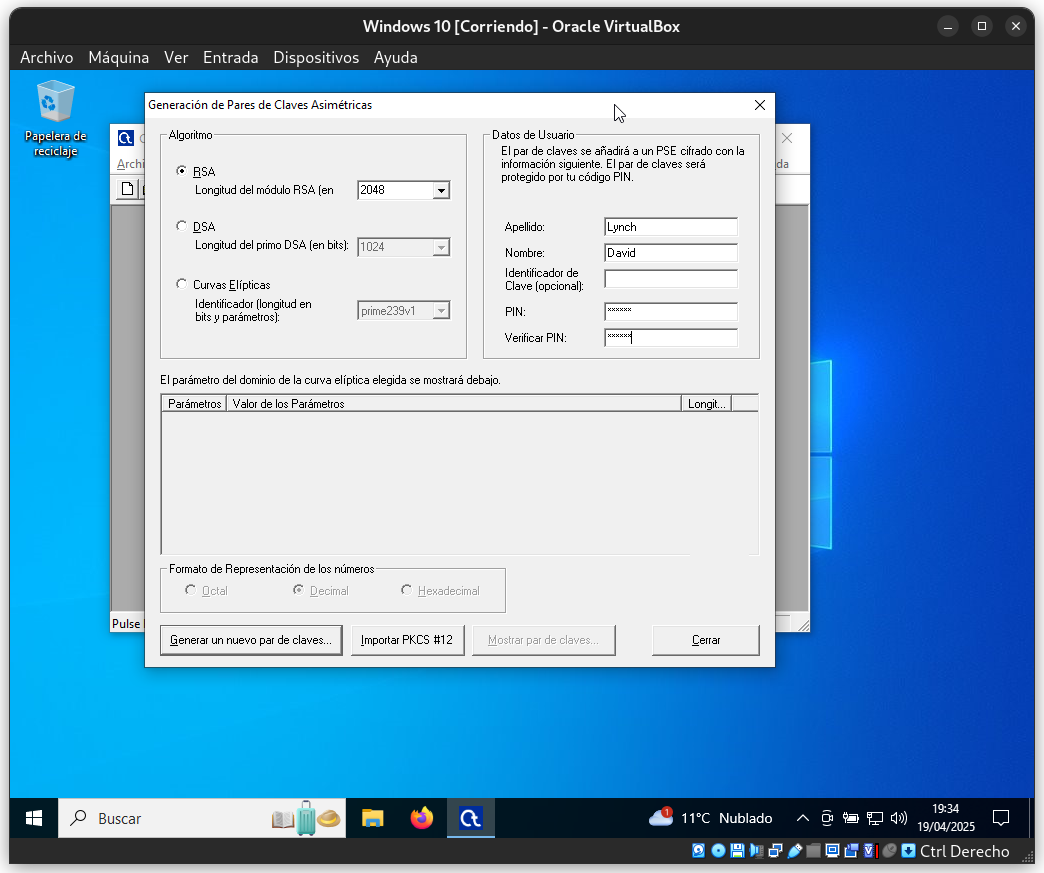
\includegraphics[width=15cm]{ClavesRSA-01.png}
    \caption{Generación del perfil del par de claves RSA}
\end{figure}

\begin{figure}[h]
    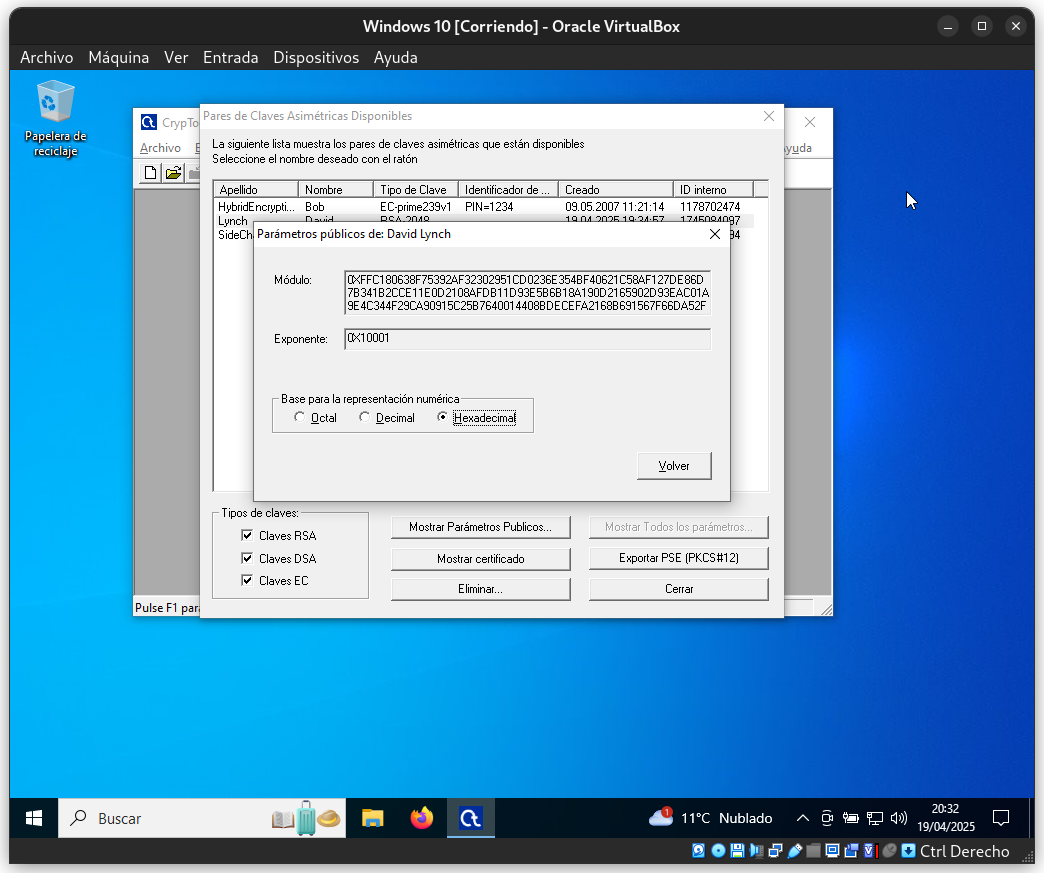
\includegraphics[width=15cm]{ClavesRSA-02.png}
    \caption{Parámetros públicos de la clave (n, e)}
\end{figure}

\begin{figure}[h]
    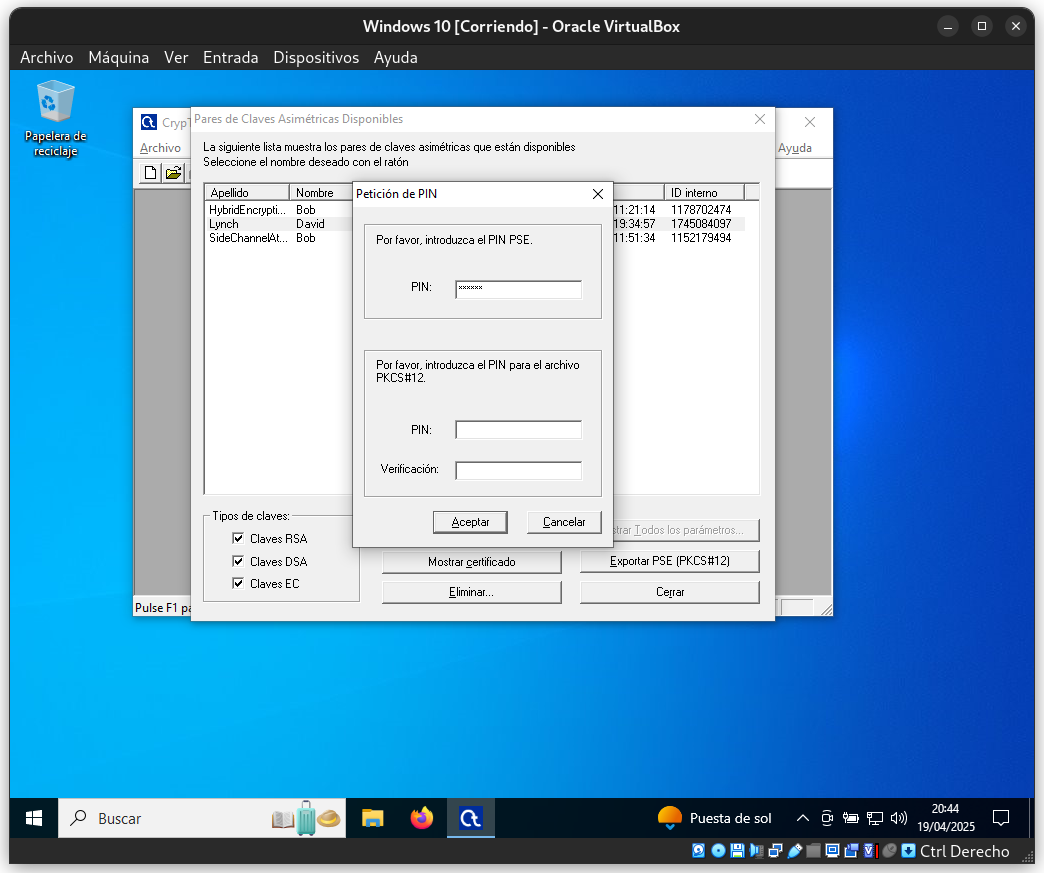
\includegraphics[width=15cm]{ClavesRSA-03.png}
    \caption{Pantalla del PIN de usuario}
\end{figure}

\begin{figure}[h]
    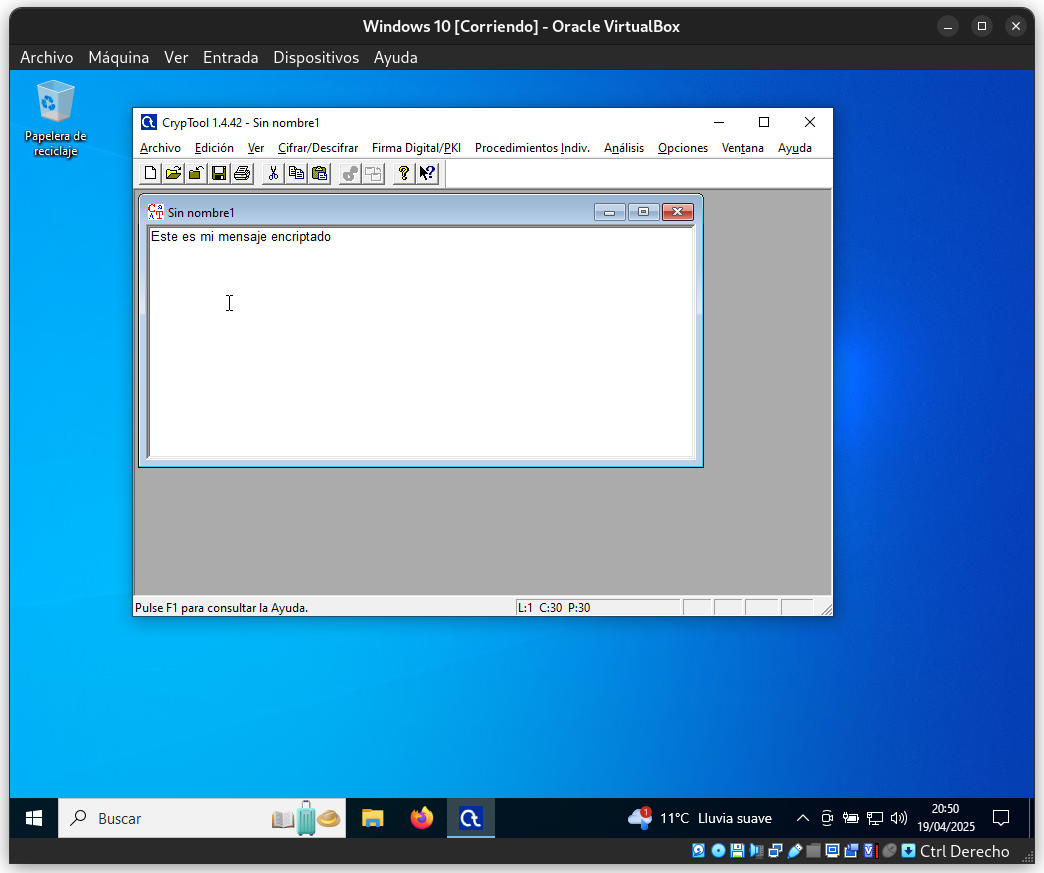
\includegraphics[width=15cm]{ClavesRSA-04.png}
    \caption{Texto de ejemplo para encriptar}
\end{figure}

\begin{figure}[h]
    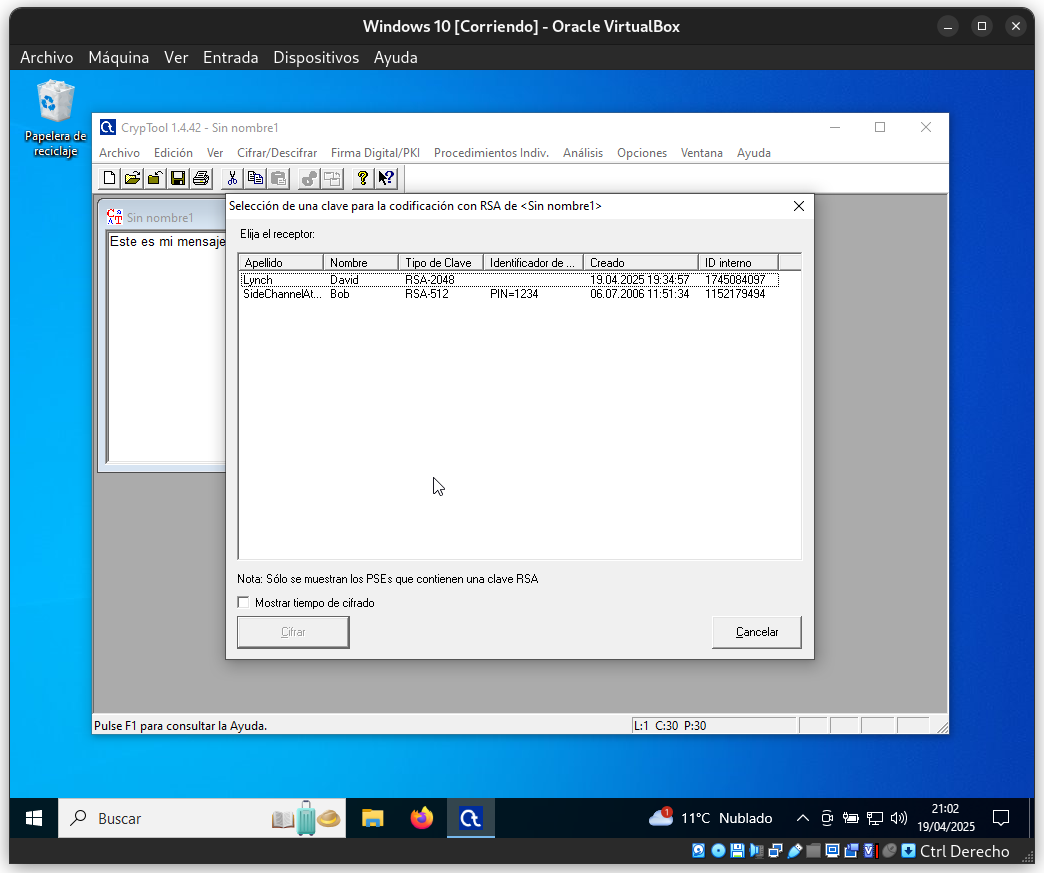
\includegraphics[width=15cm]{ClavesRSA-05.png}
    \caption{Generación del perfil del par de claves RSA}
\end{figure}

\begin{figure}[h]
    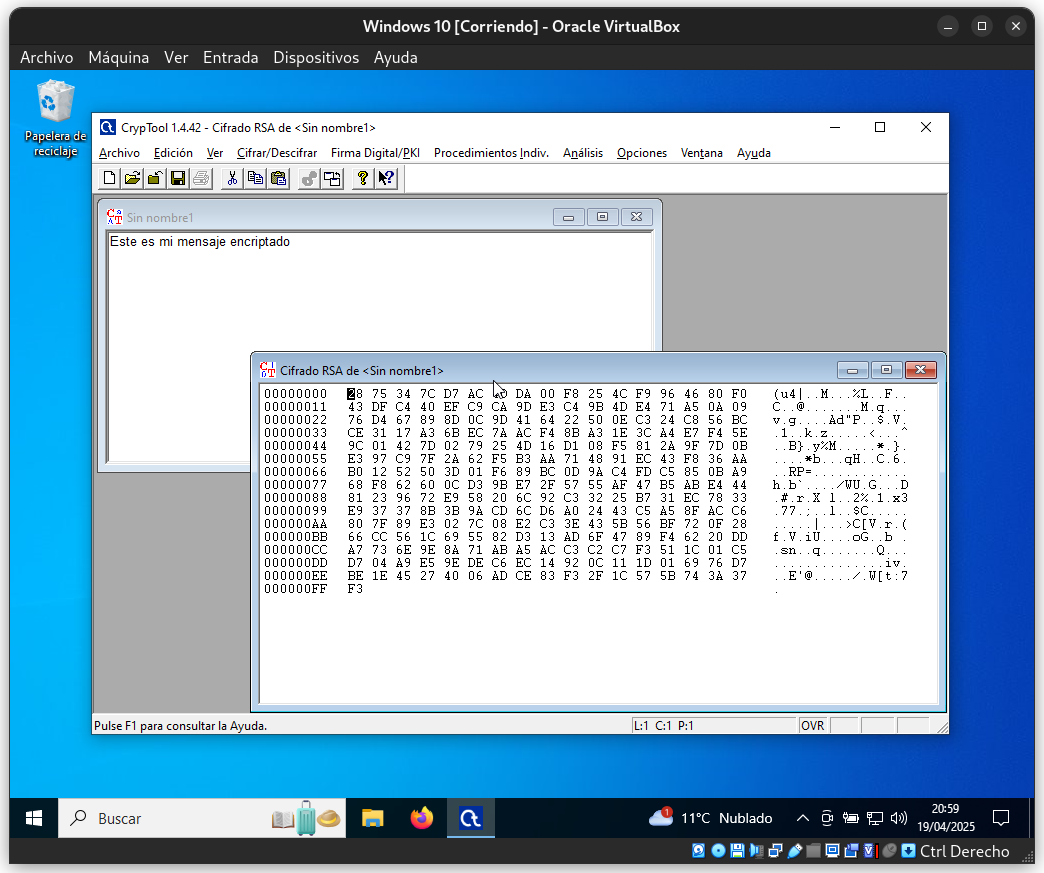
\includegraphics[width=15cm]{ClavesRSA-06.png}
    \caption{Generación del perfil del par de claves RSA}
\end{figure}

\begin{figure}[h]
    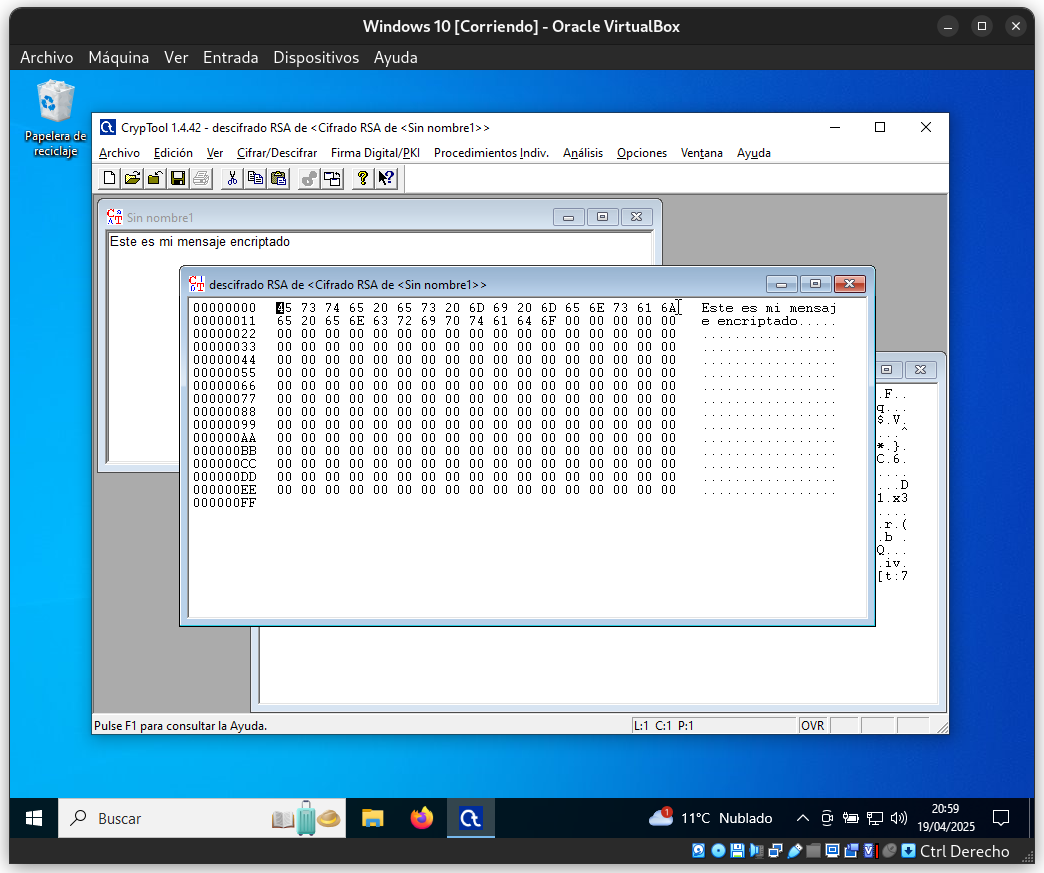
\includegraphics[width=15cm]{ClavesRSA-07.png}
    \caption{Generación del perfil del par de claves RSA}
\end{figure}

\begin{figure}[h]
    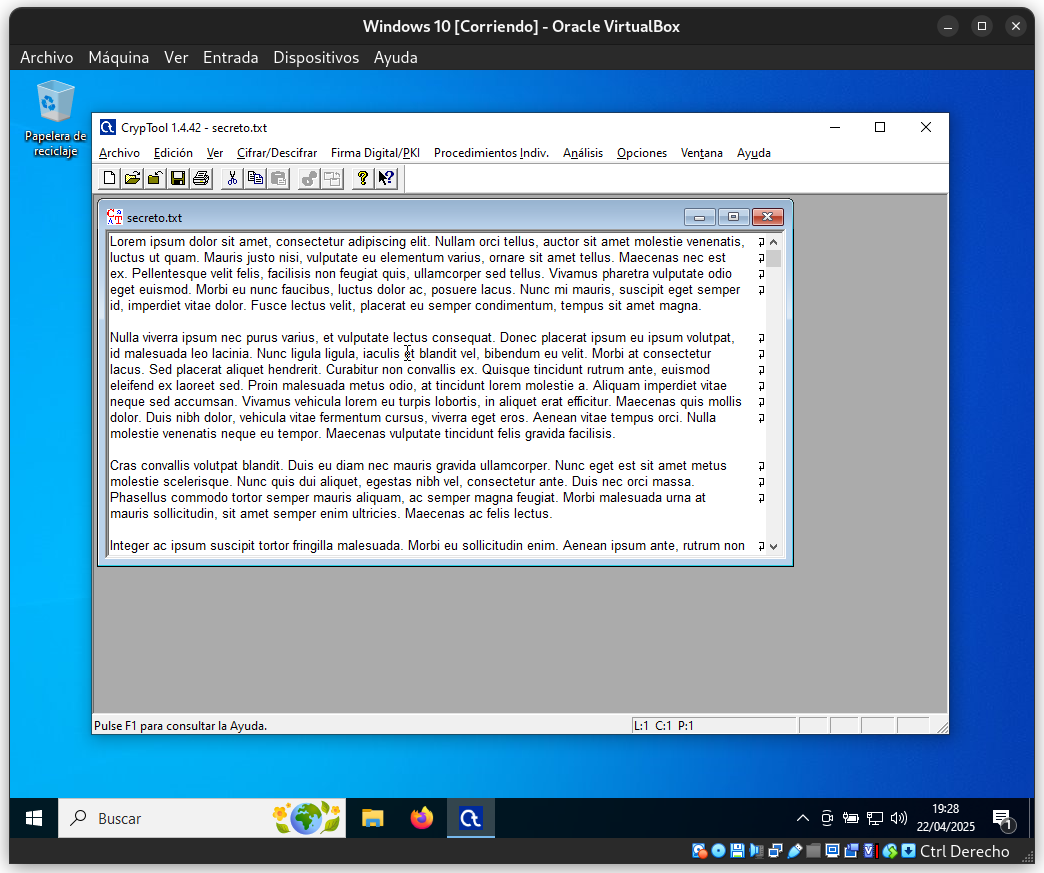
\includegraphics[width=15cm]{EncriptadoRSA-1}
    \caption{Generación del perfil del par de claves RSA}
\end{figure}

\begin{figure}[h]
    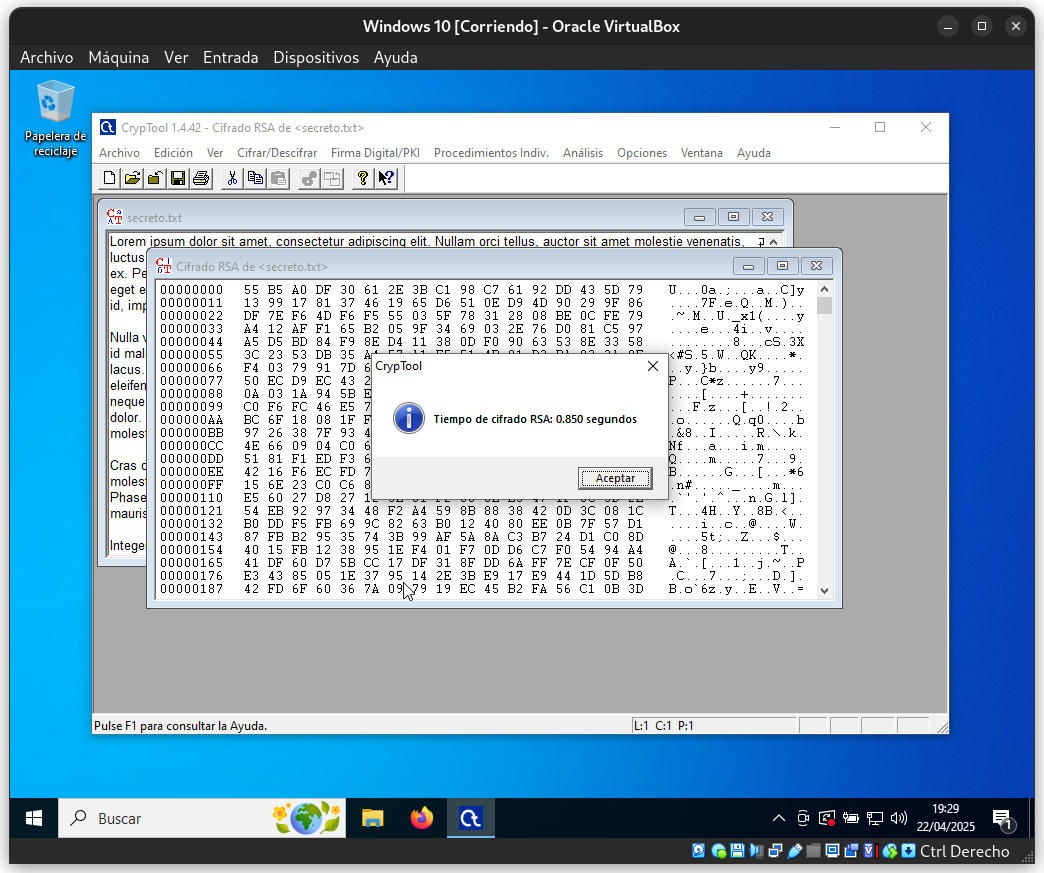
\includegraphics[width=15cm]{EncriptadoRSA-2}
    \caption{Generación del perfil del par de claves RSA}
\end{figure}

\begin{figure}[h]
    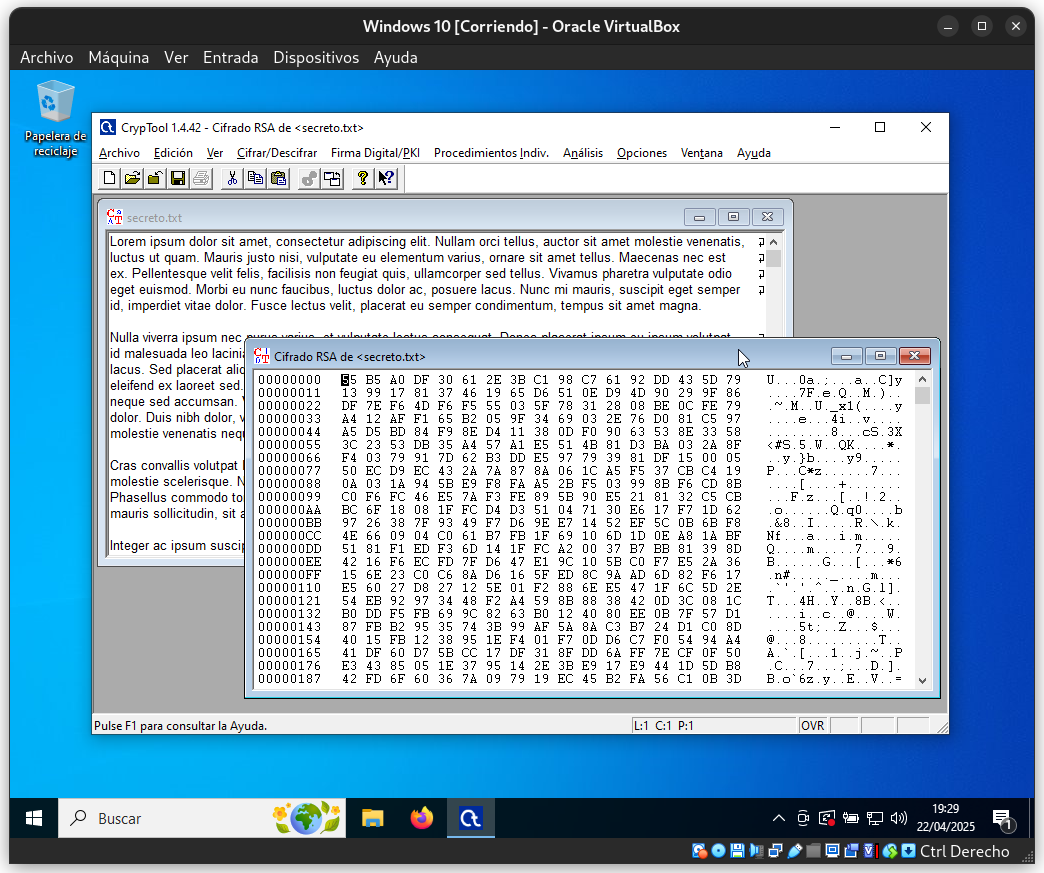
\includegraphics[width=15cm]{EncriptadoRSA-3}
    \caption{Generación del perfil del par de claves RSA}
\end{figure}

\begin{figure}[h]
    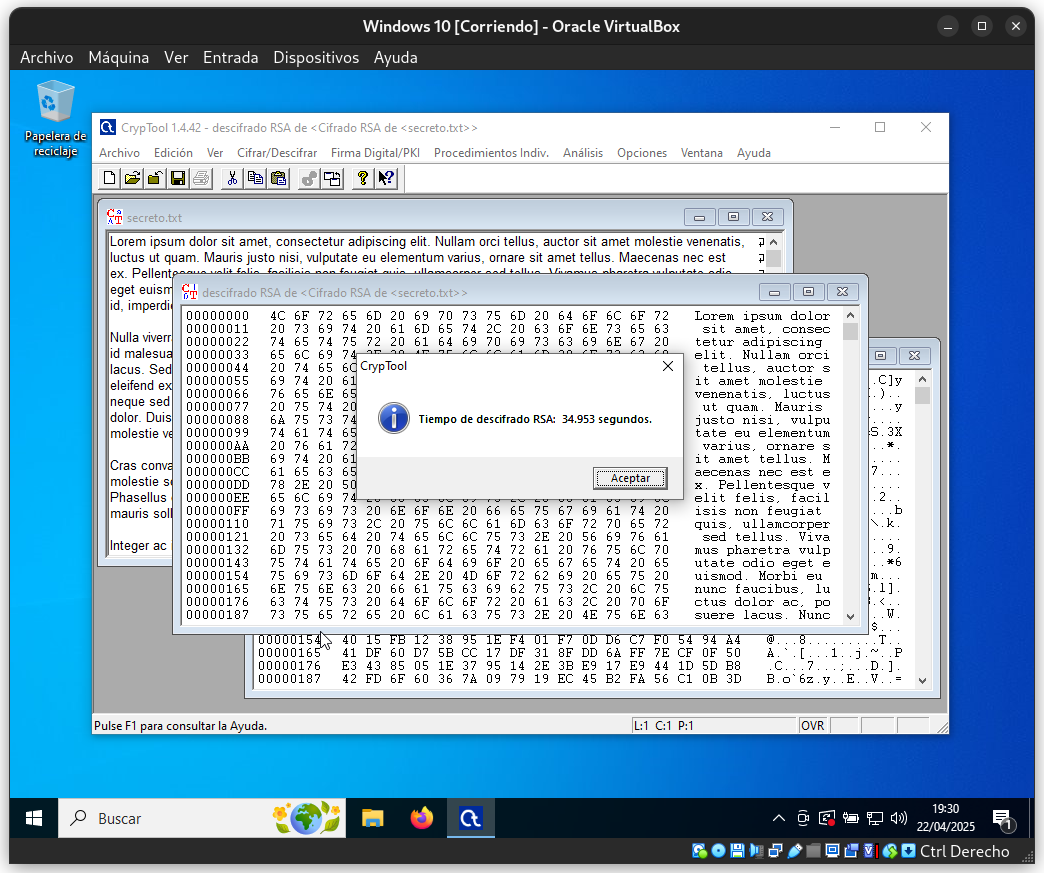
\includegraphics[width=15cm]{DesencriptadoRSA-1}
    \caption{Generación del perfil del par de claves RSA}
\end{figure}

\begin{figure}[h]
    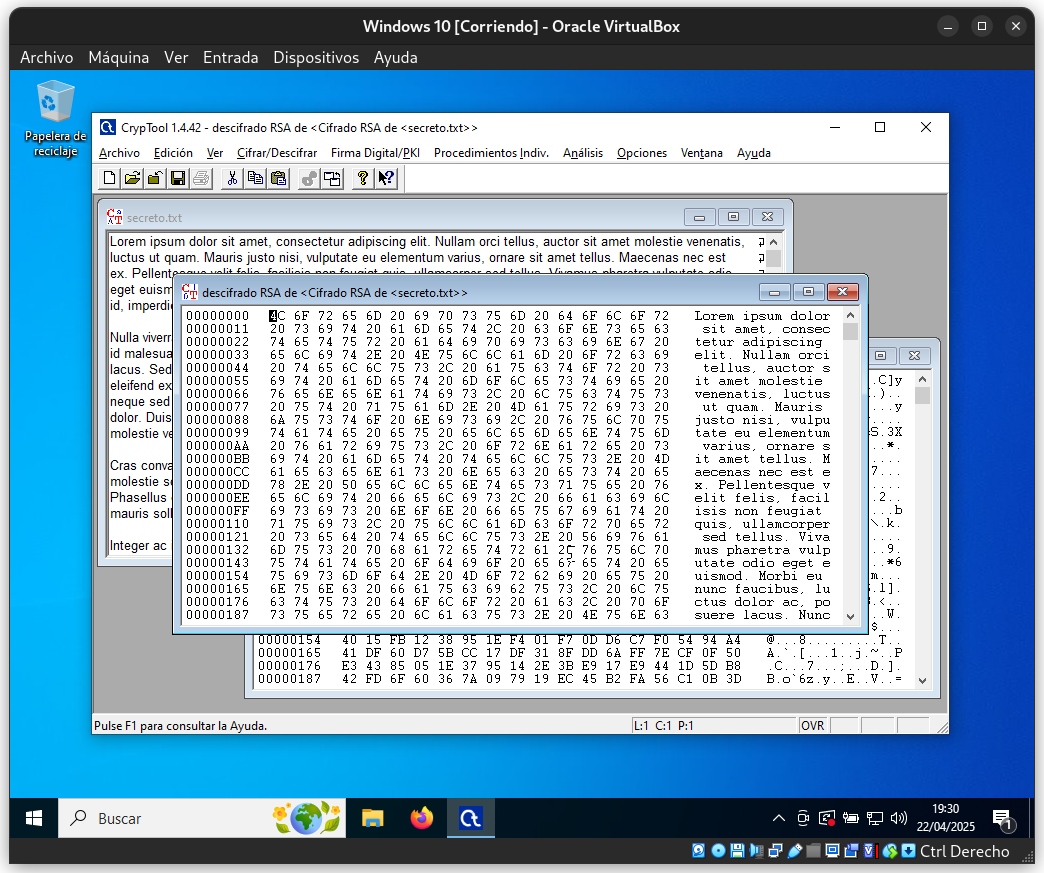
\includegraphics[width=15cm]{DesencriptadoRSA-2}
    \caption{Generación del perfil del par de claves RSA}
\end{figure}

